\documentclass[11pt]{article}
\usepackage[utf8]{inputenc}
\usepackage[T1]{fontenc}
\usepackage{amsmath}
\usepackage{amssymb}
\usepackage{booktabs}
\usepackage{graphicx}
\usepackage{geometry}
\usepackage{hyperref}
\usepackage{xurl}
\usepackage{tabularx}
\geometry{margin=1in}
\makeatletter\setlength{\@fptop}{0pt}\makeatother
\emergencystretch=2em
\newcolumntype{Y}{>{\raggedright\arraybackslash}X}
\hypersetup{colorlinks=true,linkcolor=blue,citecolor=blue,urlcolor=blue}
\title{External structural disturbance is associated with increased low-acceleration residual scatter in SPARC galaxies: a residual-blind audit}
\author{Jozsef Olcsak}
\date{May 14, 2026}
\begin{document}
\maketitle
\begin{abstract}
We present a residual-blind phenomenological audit of low-acceleration SPARC rotation-curve residual scores. Coherence labels were assigned from source-backed external evidence, frozen before residual audit, and compared against a fixed rms-log endpoint. In the quality-selected sample, the primary C-minus-A median difference for the fixed low-acceleration residual score is 0.08427, with one-sided permutation p = 0.00100 and bootstrap 95\% CI [0.04481, 0.15990]. The signal remains positive in leave-one-out, radius common-support, radius-matched, distance-matched, and distance-stratified controls. Effect-size checks show moderate A/C separation for the fixed score (AUC = 0.771) and for MOND/RAR-like baselines (AUC = 0.721-0.731), but not for the Newtonian baryonic baseline (AUC = 0.506). Residual distance/radius imbalance and observability systematics remain important caveats. The result is therefore a residual-disturbance phenomenology audit, not a unique model-selection result.

\end{abstract}
\section{Motivation}
The central question is whether external, residual-blind structural disturbance carries information about a fixed SPARC residual-scatter endpoint. If the endpoint is sensitive to real astrophysical disturbance rather than only fitting noise or post-hoc grouping, externally disturbed galaxies should show larger scatter than externally regular disks.

The study avoids optimizing labels against residuals. The primary contrast is set before the audit: quality-selected C galaxies minus quality-selected A galaxies, measured by median rms-log residual with a one-sided greater alternative. B-labeled galaxies remain useful for trend and secondary checks, but the primary endpoint is the clean A/C separation. This design keeps the study closer to a residual-blind audit than to a morphology-assisted refit, and it makes a null result possible in the usual statistical sense.

\section{Related Work And Context}
SPARC is a widely used rotation-curve and mass-model data set for nearby disk galaxies, combining 3.6 micron photometry with HI/Halpha rotation curves. It is also central to radial-acceleration-relation work, where observed centripetal acceleration correlates tightly with the baryonic acceleration inferred from the observed mass distribution. These results motivate low-acceleration residual scores as meaningful phenomenological objects, but they do not remove the need for disturbance and systematics checks.

The present study is closest to residual auditing and data-quality phenomenology. It is not a dark-matter halo fit, a full MOND test, or a derivation of a new gravitational law; it asks whether external structure information separates residual scatter after the score and labels are frozen. This framing is deliberately conservative, but it makes the result easier to compare with other residual scores and future resolved-HI samples. It also separates the present phenomenological audit from the broader projection program that originally motivated the fixed score.

Relevant observational issues include HI asymmetry, lopsidedness, non-circular motions, pressure support, asymmetric drift, beam smearing, and line-of-sight integration. HI asymmetry and lopsidedness are common enough in disk samples that they cannot be treated as rare pathologies. Three-dimensional tilted-ring modelling and LITTLE THINGS analyses show that such effects can materially affect recovered circular speeds in low-mass systems. The paper therefore reports distance, radius, inclination, velocity-error, Hubble-type, effect-size, and controlled-regression stress checks, treating unresolved observability as a limitation rather than as a solved nuisance.

\section{Fixed Residual Model}
The residual prescription is treated as a fixed model, not as a fitted galaxy-by-galaxy discovery model. It was originally motivated by a broader projection-based program, but the present paper evaluates only the frozen, reproducible residual score. A reader does not need to accept the broader theory to evaluate the audit below, because the operational question is simply whether this fixed score carries external structural information. The coefficient $\alpha$ = 0.360 is therefore not re-estimated here and should be read as part of the frozen score definition, not as a fitted claim of this paper.

For each SPARC radius point, the baryonic Newtonian speed scale is computed from the gas, disk, and bulge terms using fixed mass-to-light factors:

\begin{equation}
V_{\rm bar}^2(R)=V_{\rm gas}(R)|V_{\rm gas}(R)|+\Upsilon_d V_{\rm disk}^2(R)+\Upsilon_b V_{\rm bulge}^2(R)
\end{equation}
with fixed disk and bulge mass-to-light factors 0.5 and 0.7. The corresponding Newtonian acceleration scale is:

\begin{equation}
a_N(R)=\frac{V_{\rm bar}^2(R)}{R}
\end{equation}
after converting from (km/s)\textasciicircum{}2/kpc to SI units. The fixed projection multiplier used in this audit is:

\begin{equation}
F_{\rm proj}(R)=1+S_\tau\alpha\ln\!\left(1+\frac{a_0}{a_N(R)}\right)
\end{equation}
The numerical constants are fixed before the audit: $\alpha$ is 0.360, the acceleration scale is 1.2e-10 m/s\textasciicircum{}2, and the coherence factor is fixed at its full value of one. The predicted speed is then:

\begin{equation}
V_{\rm model}(R)=F_{\rm proj}(R)V_{\rm bar}(R)
\end{equation}
The pointwise log residual and galaxy-level endpoint are:

\begin{equation}
\epsilon_i=\ln\!\left(\frac{V_{{\rm obs},i}}{V_{{\rm model},i}}\right)
\end{equation}
\begin{equation}
{\rm rms}_{\log}=\left(\frac{1}{N}\sum_i\epsilon_i^2\right)^{1/2}
\end{equation}
The formula is a fixed working prescription set in code before the residual-blind label audit. It is framed here as a reproducible residual score, not as a fully derived physical theory.

\subsection{Model Motivation}
The model starts from the standard SPARC baryonic decomposition rather than from observed residuals. The only additional ingredient is a fixed multiplicative correction depending on the local baryonic acceleration scale.

\subsection{Rationale For The Logarithmic Ansatz}
The logarithmic form of \texttt{F\_proj} is not used as arbitrary curve-fitting convenience. It was chosen instead of a power-law boost because it remains stable in the ultra-low-acceleration regime: the correction can grow where \texttt{a\_N << a0}, but only logarithmically. It also preserves a smooth baryonic limit at high acceleration, where the logarithmic correction tends toward zero.

This choice is motivated by the broader projection picture behind the fixed score: scale-free geometric projection effects suggest dependence on ratios of acceleration scales rather than on an added absolute acceleration. A logarithm of \texttt{1 + a0/a\_N} is a minimal way to encode such a ratio while preserving a smooth baryonic limit at high acceleration. In this paper that motivation defines a fixed dynamical score; it is not used as a complete derivation of the underlying theory. The audit therefore tests an operational consequence of the score, not the full theoretical program.

The acceleration scale is fixed at the familiar low-acceleration value used in galaxy-dynamics phenomenology, and $\alpha$ = 0.360 is treated as a fixed model constant. Neither is fitted in the residual-blind label audit. The coherence factor is set to one, so no galaxy-specific coherence parameter is tuned to improve individual fits. The coefficient and ansatz are therefore part of the pre-frozen score; their deeper theoretical motivation is left to a companion model note.

The test is intentionally narrow: if the frozen endpoint is sensitive to structural disturbance, externally disturbed or coherence-poor galaxies should tend to have larger residual scatter than externally regular disks.

The analysis has four fixed steps:

\begin{enumerate}
\item Compute SPARC residual summaries under the fixed low-acceleration prescription.
\item Assign external coherence labels without inspecting those residual summaries.
\item Freeze the quality selection, labels, endpoint, and primary contrast.
\item Test whether quality-selected C galaxies have higher rms-log residual scatter than quality-selected A galaxies.
\end{enumerate}

\begin{figure}[htbp]
\centering
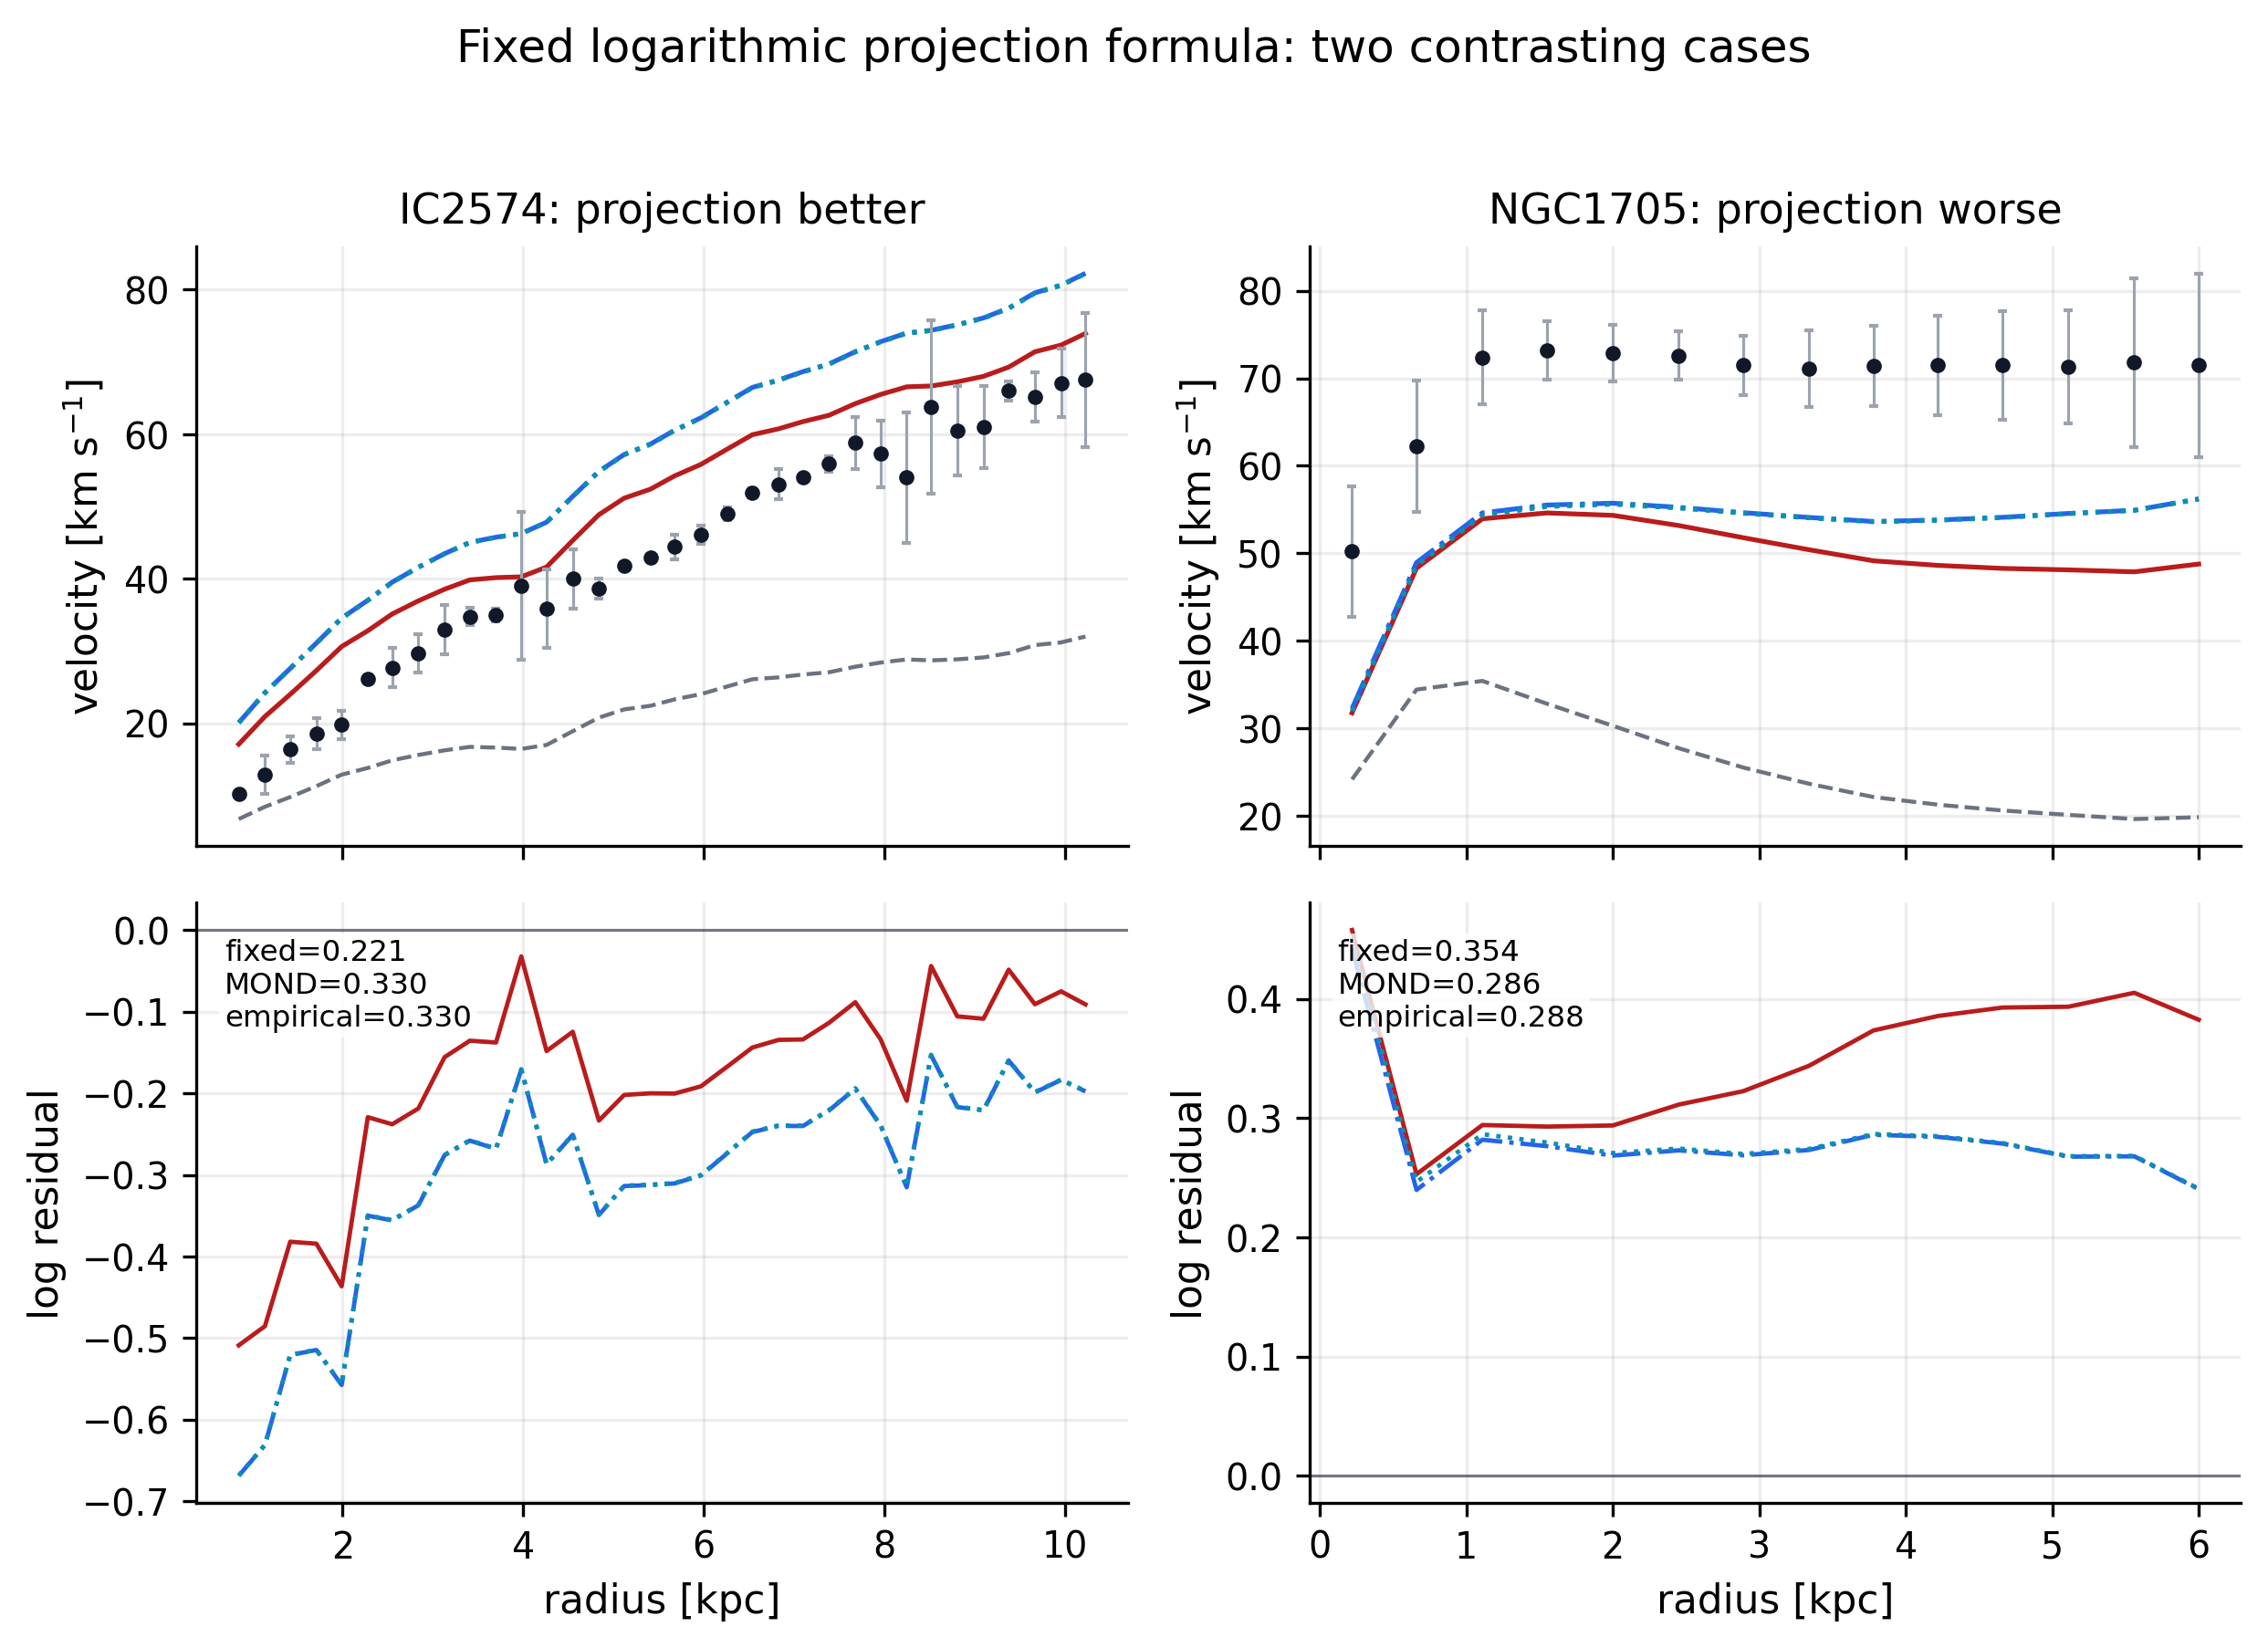
\includegraphics[width=0.88\linewidth]{figures/projection_vs_mond_rotation_examples.png}
\caption{Fixed logarithmic projection formula compared with MOND/RAR-family baselines on two contrasting SPARC rotation curves. IC2574 illustrates a case where the fixed projection score has lower rms-log residual than the MOND/RAR-like baselines; NGC1705 illustrates the opposite. These examples are selected only to show model behavior around the logarithmic ansatz introduced above. They are not used as endpoints, tuning targets, or evidence for uniqueness over MOND/RAR-family scores. No separate numerical RMOND model is evaluated in this packet.}
\label{fig:projection_vs_mond_rotation_examples}
\end{figure}

\begin{figure}[htbp]
\centering
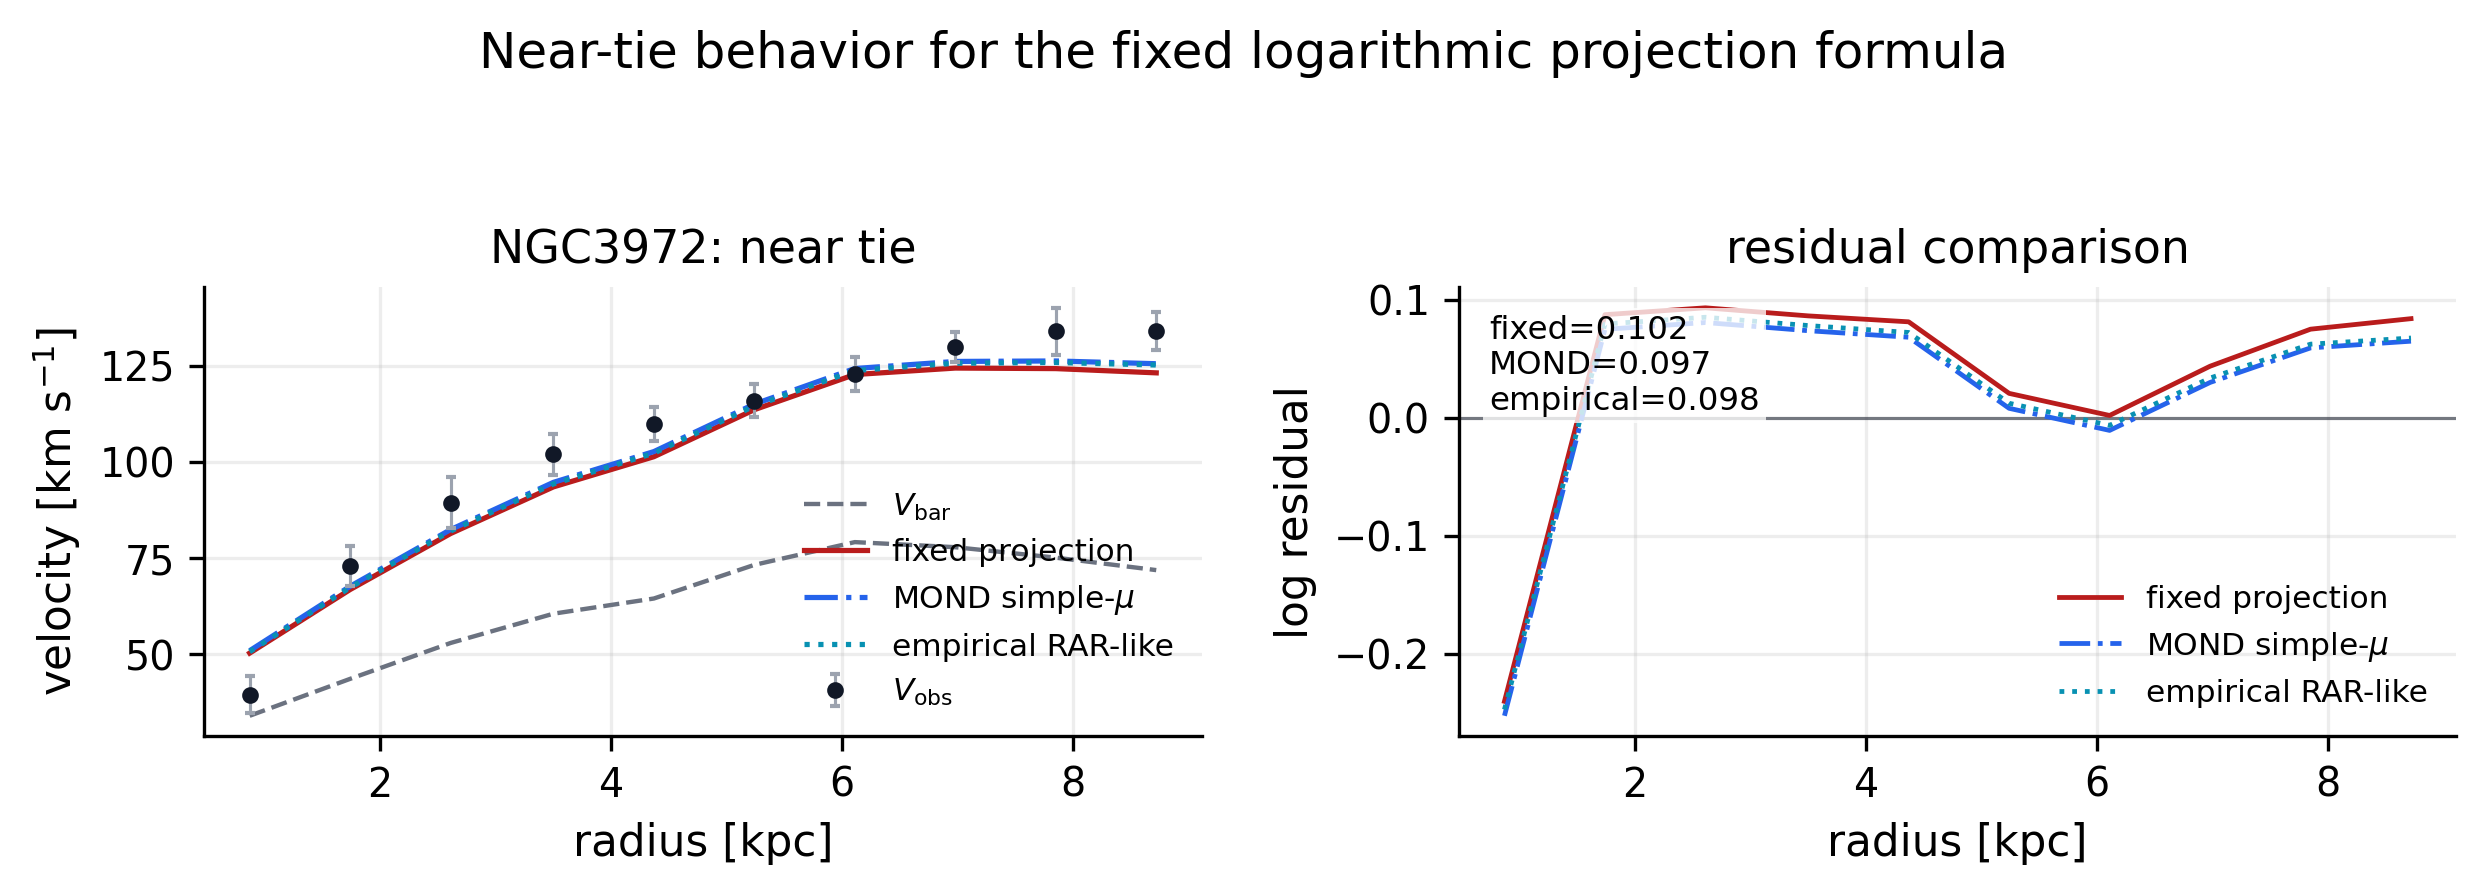
\includegraphics[width=0.82\linewidth]{figures/projection_vs_mond_near_tie_example.png}
\caption{Near-tie behavior for NGC3972. In this case the fixed projection, MOND simple-$\mu$, and empirical RAR-like curves give very similar residual scales, illustrating why the paper treats the fixed logarithmic prescription as an operational score rather than as a unique model-selection result.}
\label{fig:projection_vs_mond_near_tie_example}
\end{figure}

\section{Data And Endpoint}
The residual source is the SPARC residual summary for the fixed low-acceleration score. The endpoint is rms-log scatter after the study quality gate, which requires sufficient rotation-curve support and diagnostic quality. The quality-selected sample contains 73 galaxies: 17 A, 28 B, and 28 C.

The primary statistic is the median difference:

\begin{equation}
\Delta_{AC}={\rm median}({\rm rms}_{\log}\mid C,{\rm selected})-{\rm median}({\rm rms}_{\log}\mid A,{\rm selected})
\end{equation}
Inference uses count-preserving label permutation for the one-sided p-value and bootstrap resampling for the confidence interval. This keeps the test aligned with the frozen A/C class sizes and avoids model-fitting degrees of freedom. The statistic is intentionally simple, because the sample is modest and the main risk is not underfitting but over-interpreting a flexible analysis.

\begin{figure}[htbp]
\centering
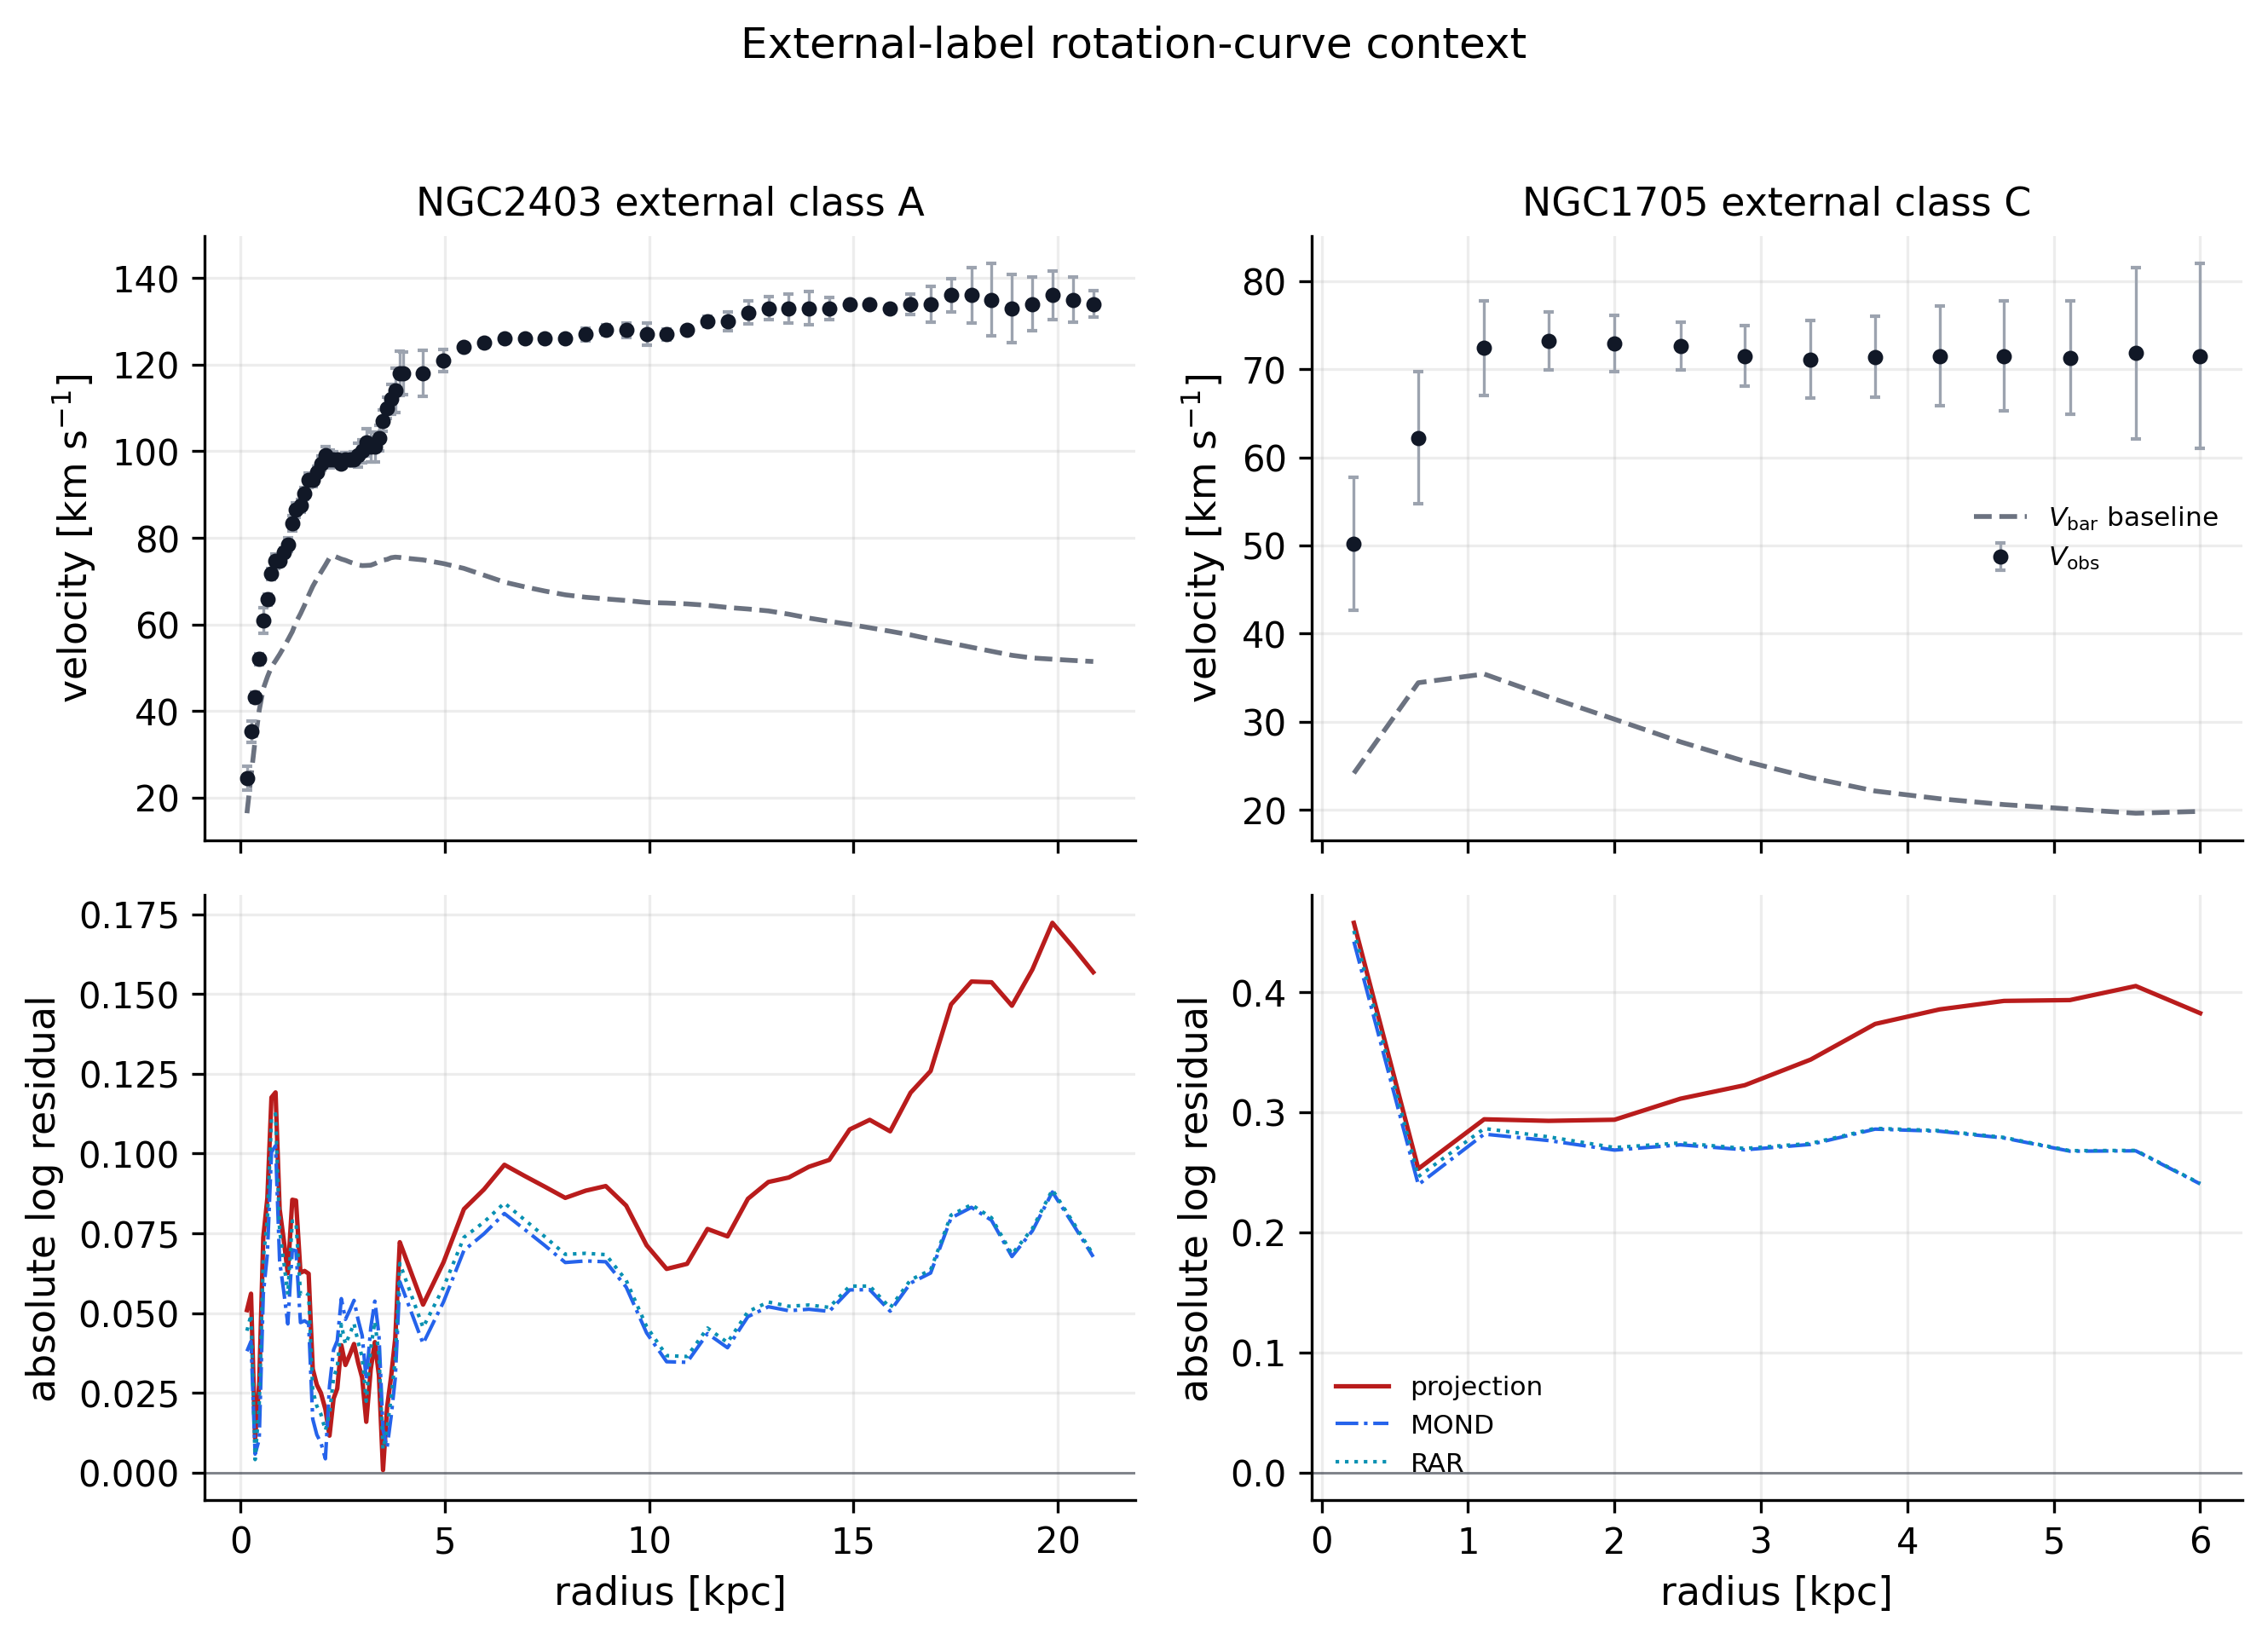
\includegraphics[width=0.94\linewidth]{figures/illustrative_rotation_curves.png}
\caption{External-label rotation-curve context for NGC2403, a regular class-A disk, and NGC1705, a disturbed class-C dwarf. The upper panels show observed rotation curves against the baryonic baseline; the lower panels show the per-radius absolute residual profiles that feed the score families. This visualization is not a primary endpoint and is not used for labeling, threshold selection, or model tuning.}
\label{fig:illustrative_rotation_curves}
\end{figure}


\section{Labeling Protocol And External Evidence}
Labels encode external structural state rather than residual behavior. Class A denotes externally regular/coherent disks, class C denotes externally disturbed or coherence-poor systems, and class B denotes uncertain or intermediate cases. The A/C evidence rows were expanded to reduce dependence on uncertain labels and to make the distance imbalance testable.

This discipline is central: the result is not that an analyst can separate high- and low-residual galaxies after inspecting residuals, but that residual-blind external evidence predicts the frozen endpoint. The packet records this audit layer in \path{labeling_protocol.md}, which defines the source rules and A/B/C decision logic, and in \path{external_evidence_table.csv}, which gives row-level evidence summaries, source links, reviewer/date fields, and residual-blind flags.

The protocol is intentionally conservative. A requires direct regular-disk evidence such as regular HI/Halpha kinematics, low asymmetry, or a well-defined symmetric rotation curve. C requires direct disturbance evidence such as disturbed HI morphology, lopsided velocity fields, tidal or interaction signatures, or warp evidence tied to gas morphology or kinematics. Environment-only, bar-only, or rotation-curve-quality-only information is not enough for an A/C call; ambiguous rows default to B. This makes some classifications less aggressive, but it reduces the risk that the final contrast is created by weak or indirect evidence.

Figure 1 shows the quality-selected residual distribution by external class. Labels are external; plotted residuals enter only after the labels are frozen.

\begin{figure}[htbp]
\centering
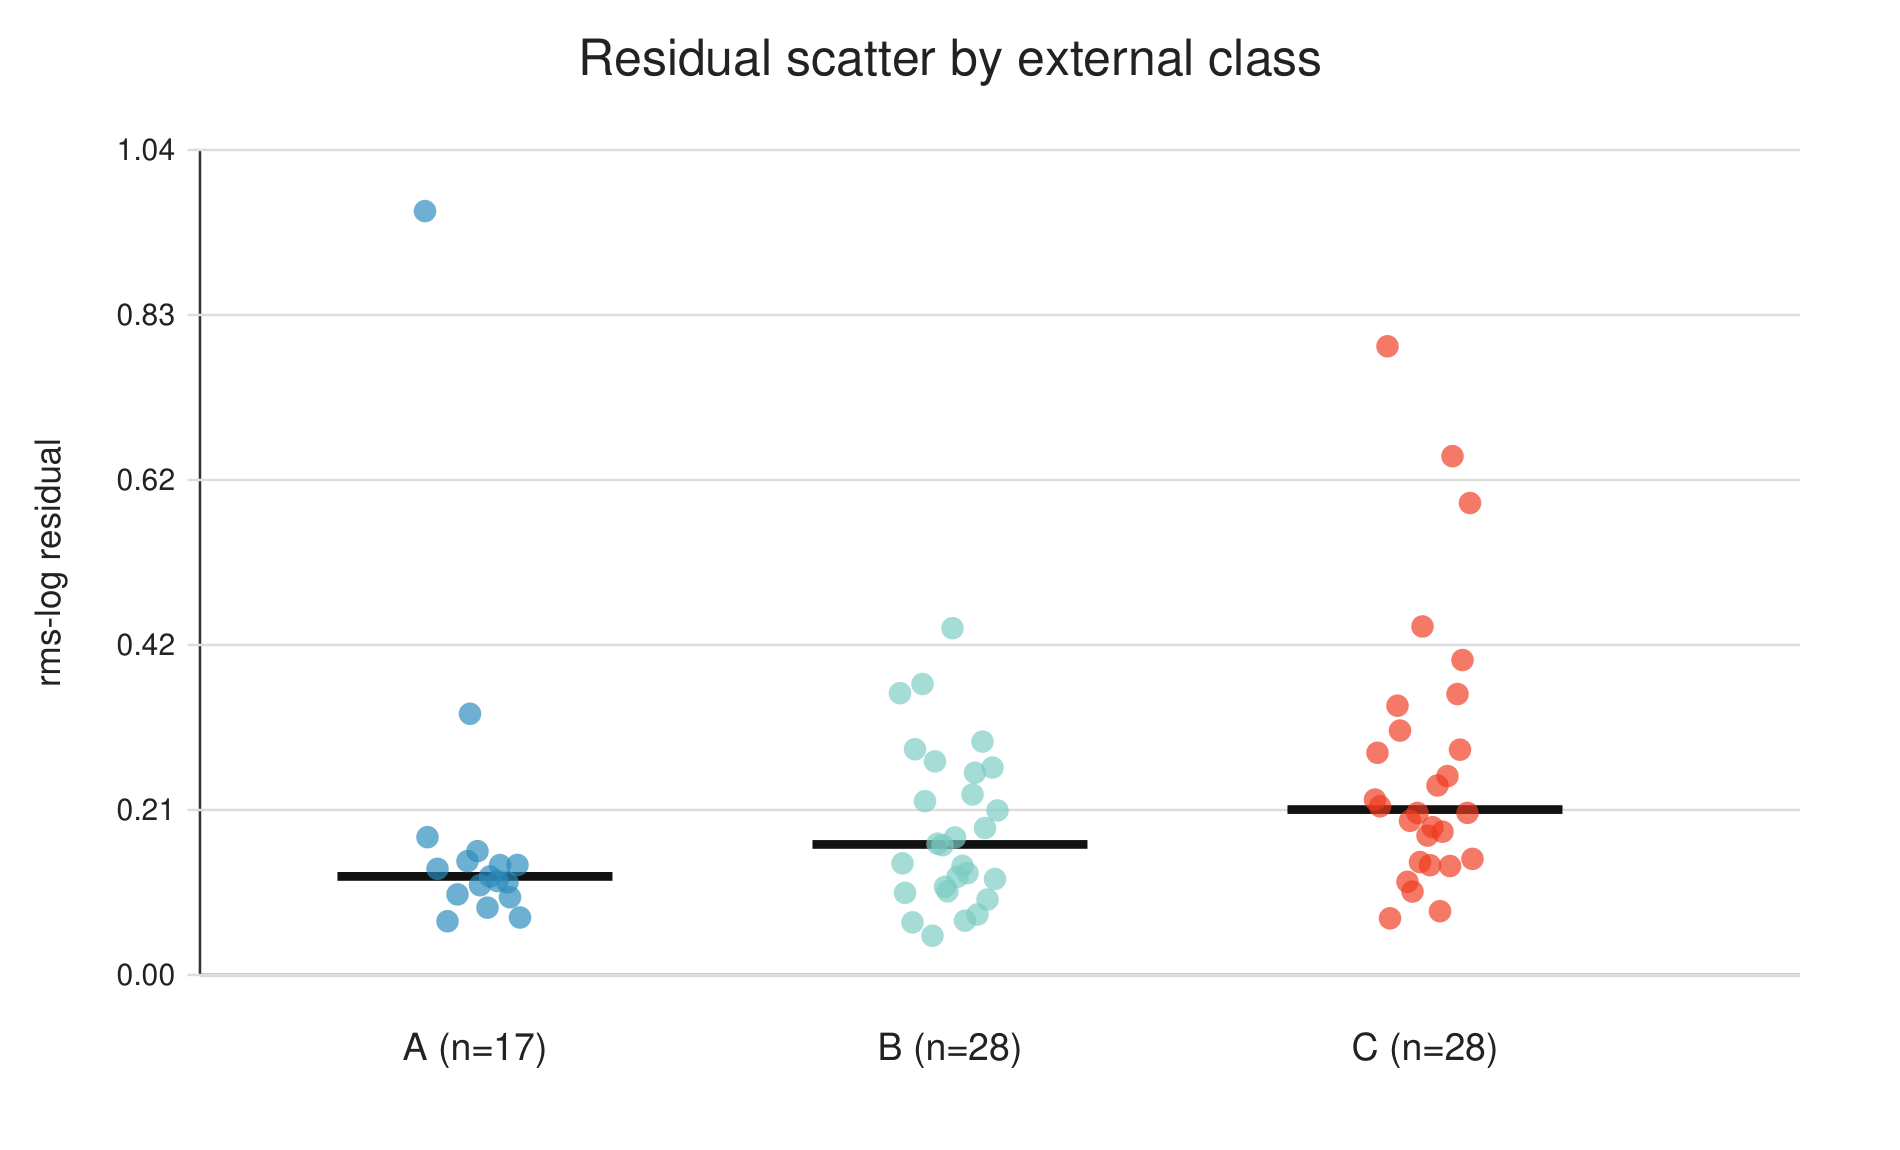
\includegraphics[width=0.86\linewidth]{figures/quality_pass_rms_distribution.png}
\caption{Residual scatter by external class.}
\label{fig:quality_pass_rms_distribution}
\end{figure}
\section{Primary Result}
The primary result is positive:

\begin{table}[htbp]
\centering
\footnotesize
\setlength{\tabcolsep}{3pt}
\begin{tabularx}{\linewidth}{Y Y Y Y Y Y Y Y Y}
\toprule
comparison & n A & n C & median A & median C & C-A diff & p & CI low & CI high \\
\midrule
quality-selected C-minus-A & 17 & 28 & 0.12436 & 0.20862 & 0.08427 & 0.00100 & 0.04481 & 0.15990 \\
\bottomrule
\end{tabularx}
\end{table}
Externally disturbed/coherence-poor galaxies have larger fixed-score residual scatter than externally regular galaxies. The bootstrap interval is fully positive and the one-sided permutation p-value is 0.00100.

The effect is not only a p-value result. A descriptive effect-size appendix gives AUC = 0.771 for the fixed low-acceleration residual score: a randomly selected C galaxy has larger fixed-score scatter than a randomly selected A galaxy in about 77\% of A/C pairs. The robust median-scaled effect is 0.938. These quantities are descriptive effect sizes for an observational audit, not estimates of a universal physical constant.

Secondary quality-selected checks support the same ordering. The C-minus-nonC contrast is positive (p = 0.0173), and the ordered A-to-B-to-C trend is positive (rho = 0.3620, p = 0.00110). The A/C leave-one-out check produces no sign flips, so the primary direction is not set by a single influential galaxy.

Figure 2 summarizes the primary result and main controls on a common effect scale.

\begin{figure}[htbp]
\centering
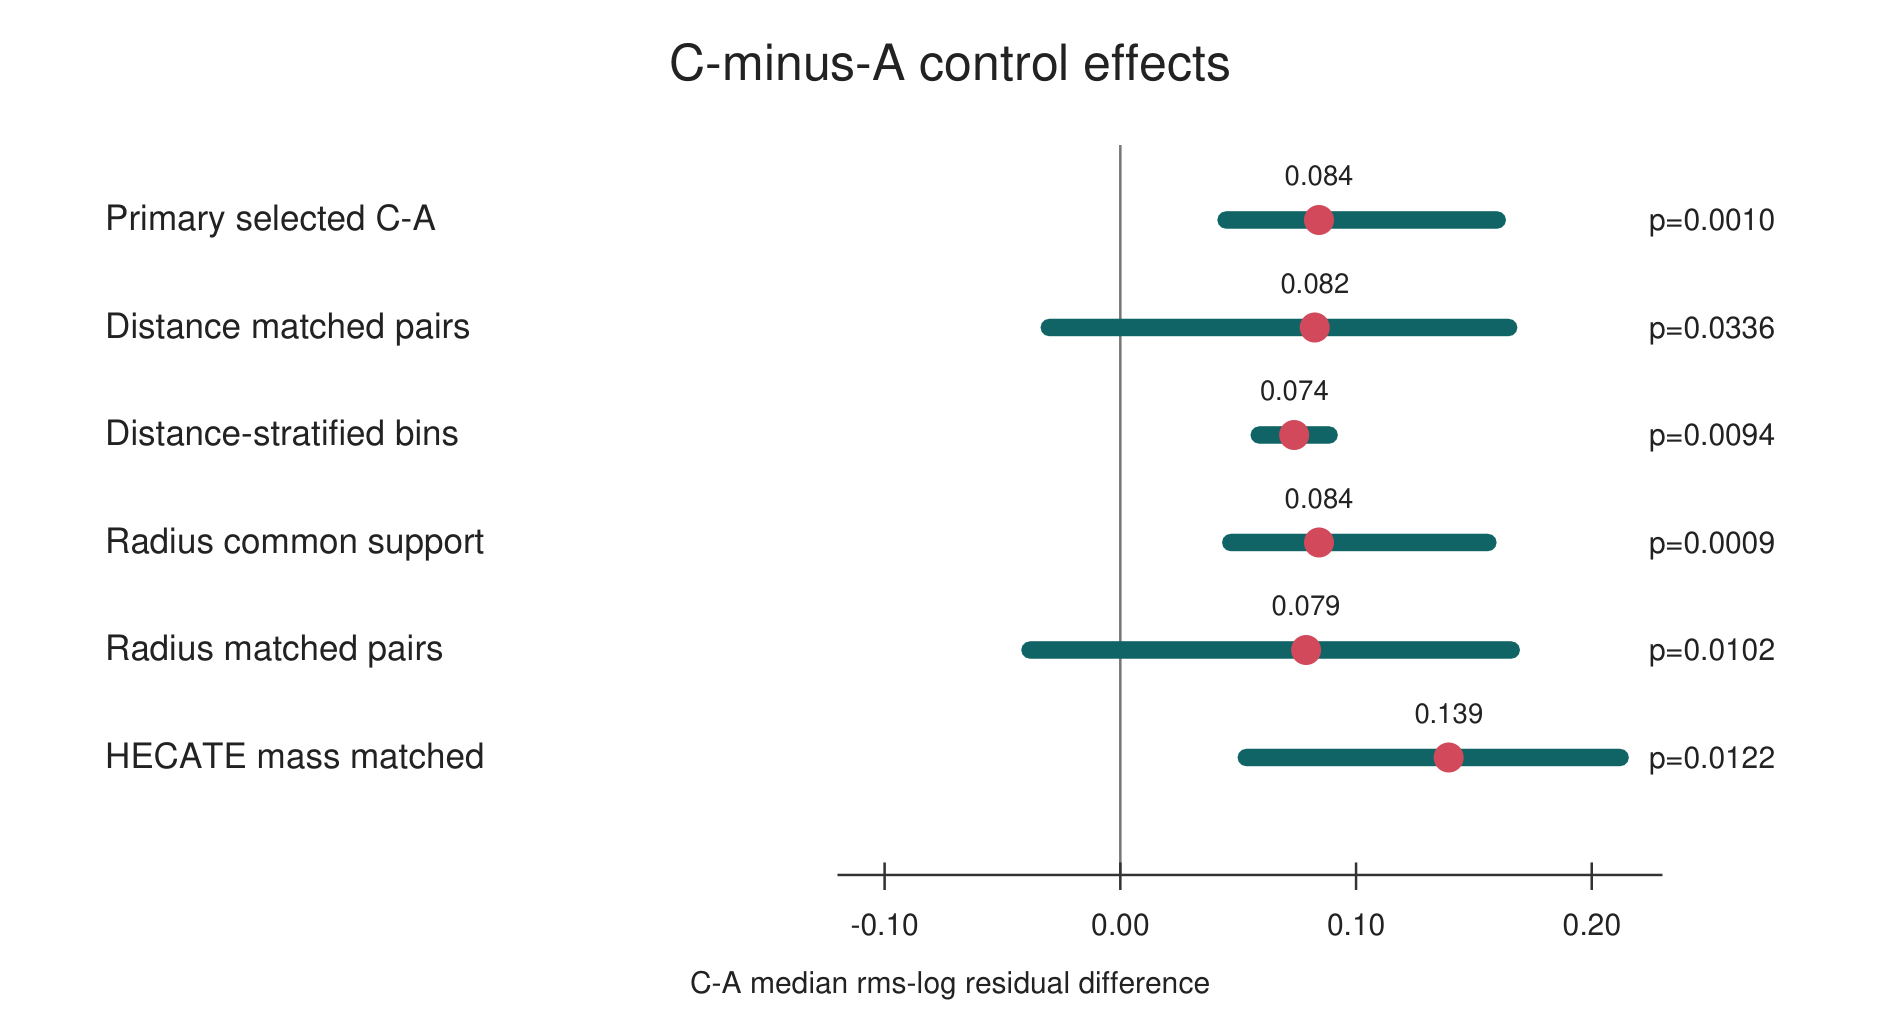
\includegraphics[width=0.86\linewidth]{figures/control_forest_plot.png}
\caption{C-minus-A control effects.}
\label{fig:control_forest_plot}
\end{figure}
\section{Distance And Scale Controls}
The main potential confound is that C galaxies are, on average, closer and smaller in radius than A galaxies. Controls reduce this concern but do not remove it. Raw SPARC distance imbalance remains visible: A median distance is 13.8 Mpc, C median distance is 7.83 Mpc, and the two-sided imbalance p-value is 0.02490. This imbalance is scientifically important because the same observability differences that make disturbance easier to identify may also change the measured rotation-curve residual structure.

The important change is that matched and stratified controls no longer collapse the signal:

\begin{table}[htbp]
\centering
\footnotesize
\setlength{\tabcolsep}{3pt}
\begin{tabularx}{\linewidth}{Y Y Y}
\toprule
control & effect & p \\
\midrule
greedy SPARC distance-matched pairs & 0.08247 & 0.03360 \\
optimal ordered SPARC distance-matched pairs & 0.08247 & 0.03610 \\
strict $\leq$2 Mpc distance caliper & 0.11949 & 0.08979 \\
distance-stratified within-bin test & 0.07374 & 0.00940 \\
\bottomrule
\end{tabularx}
\end{table}
Every distance bin has a positive C-minus-A median difference:

\begin{table}[htbp]
\centering
\footnotesize
\setlength{\tabcolsep}{3pt}
\begin{tabularx}{\linewidth}{Y Y Y Y}
\toprule
SPARC distance bin & n A & n C & C-A diff \\
\midrule
0-5 Mpc & 3 & 10 & 0.07409 \\
5-10 Mpc & 4 & 10 & 0.06147 \\
10-20 Mpc & 7 & 6 & 0.08512 \\
>20 Mpc & 3 & 2 & 0.06361 \\
\bottomrule
\end{tabularx}
\end{table}
Figure 3 shows the same within-bin result visually.

\begin{figure}[htbp]
\centering
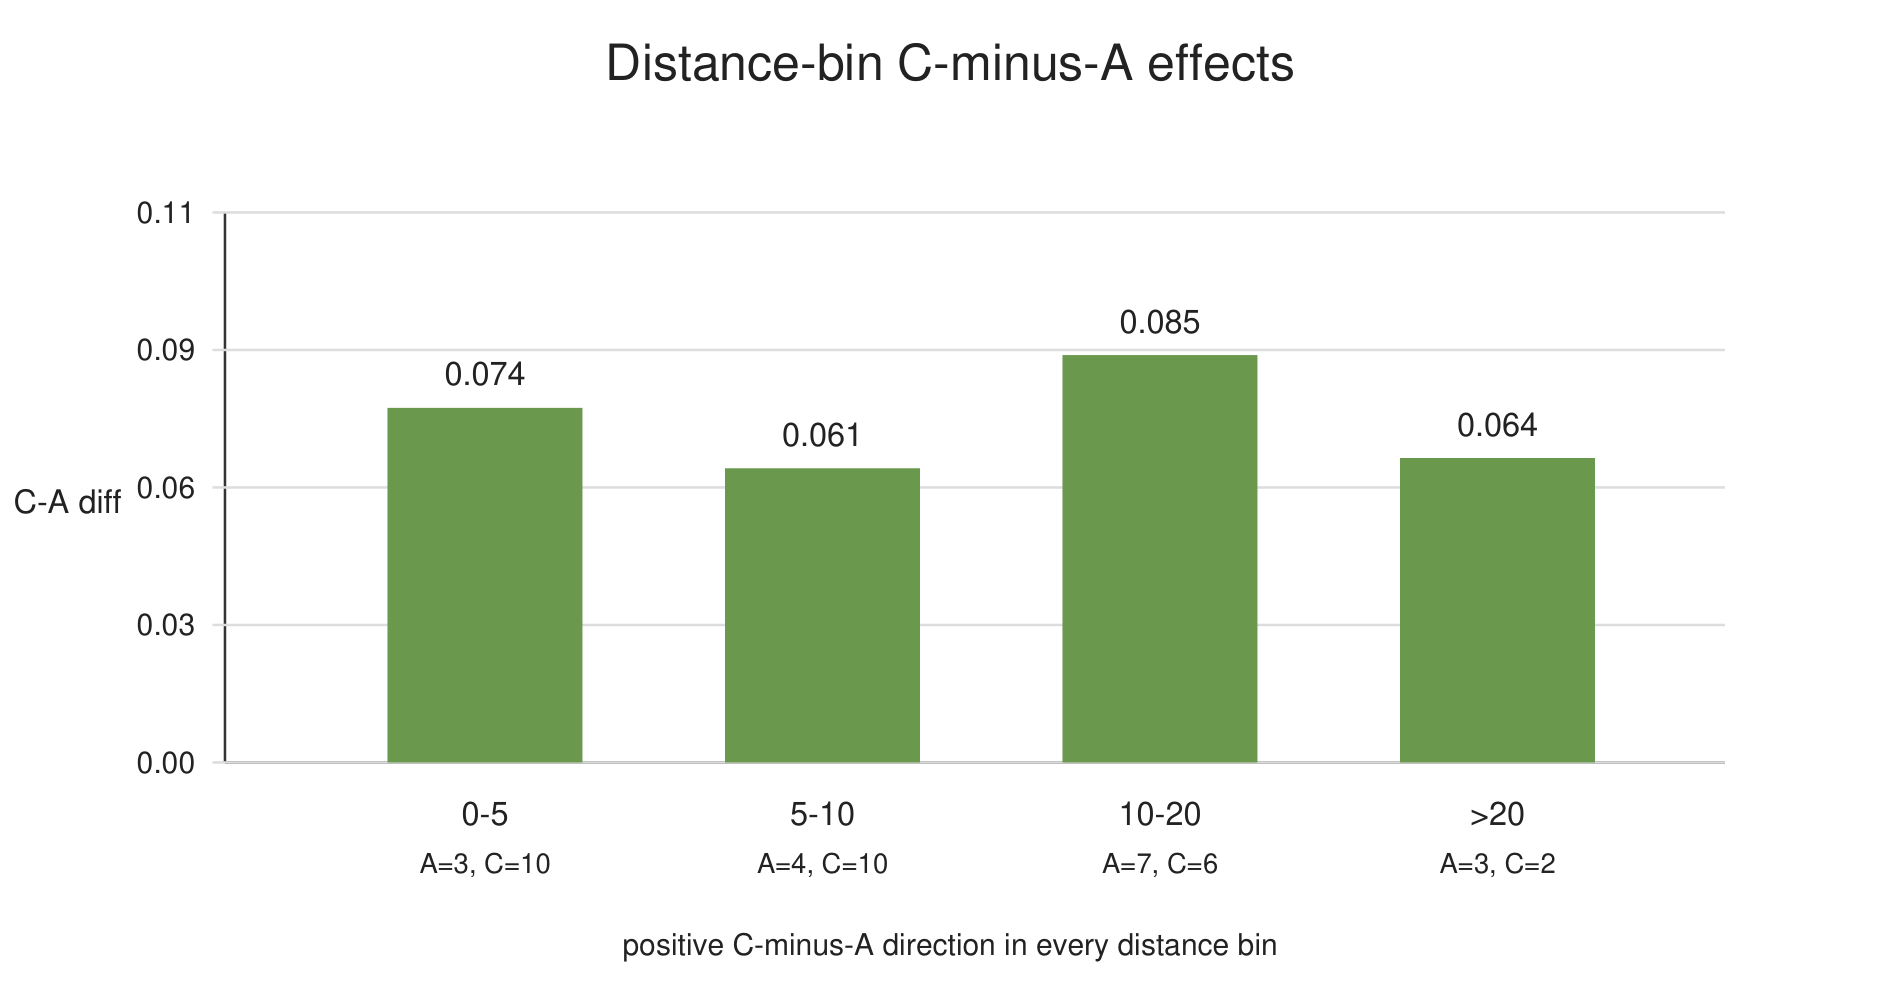
\includegraphics[width=0.86\linewidth]{figures/distance_stratified_effects.png}
\caption{Distance-bin effects.}
\label{fig:distance_stratified_effects}
\end{figure}
Radius controls also preserve the predicted direction. The max-radius imbalance remains visible (p = 0.00190), but common-support and greedy radius-matched tests are positive (p = 0.00090 and p = 0.01020); the strict $\leq$2 kpc caliper is positive but underpowered (p = 0.10969). Thus the radius checks support the same direction, while also showing that very strict matching quickly reduces sample support.

HECATE stellar-mass matching is directionally supportive where coverage exists (p = 0.01220 and p = 0.01440), but incomplete dwarf-regime coverage makes it supplementary.

The selection/observability appendix records distance, distance uncertainty, radial coverage, point count, velocity-error, inclination, Hubble-type, WHISP-family coverage, and partial HECATE mass balance. A robust regression stress test is positive in class-only and distance-only specifications, weakens after distance and radial coverage are included together, and remains positive but not bootstrap-exclusive of zero in the full observability specification. This is an important constraint on the claim: the signal is directionally stable across several controls, but it is not yet an observability-proof physical detection.

Threshold-sensitivity and weighted-residual figures are useful supplementary diagnostics, but they repeat the same class-ordering message rather than testing the main confound.

\section{Alternative Baseline Scores}
The same residual-blind A/C labels were compared against three alternative baseline scores from the same SPARC rotmod rows and fixed mass-to-light factors. These are not replacement endpoints; they test whether class separation is specific to the frozen low-acceleration score or reflects broader disturbance sensitivity.

\begin{table}[htbp]
\centering
\footnotesize
\setlength{\tabcolsep}{3pt}
\begin{tabularx}{\linewidth}{Y Y Y Y Y Y Y Y Y}
\toprule
score & n A & n C & median A & median C & C-A diff & p & CI low & CI high \\
\midrule
fixed score & 17 & 28 & 0.12436 & 0.20862 & 0.08427 & 0.00210 & 0.04440 & 0.15792 \\
Newtonian baryonic & 17 & 28 & 0.57056 & 0.61615 & 0.04559 & 0.39546 & -0.20123 & 0.31376 \\
MOND simple-mu & 17 & 28 & 0.11366 & 0.23238 & 0.11872 & 0.00190 & 0.00305 & 0.17644 \\
empirical RAR & 17 & 28 & 0.11360 & 0.22442 & 0.11082 & 0.00210 & 0.00583 & 0.17395 \\
\bottomrule
\end{tabularx}
\end{table}
The Newtonian baryonic baseline is not a significant separator. MOND-like and empirical RAR baselines show positive A/C separation, so the result should not be described as uniqueness evidence for the projection formula. The effect-size comparison sharpens this: fixed score AUC = 0.771, MOND simple-mu AUC = 0.721, empirical RAR AUC = 0.731, and Newtonian baryonic AUC = 0.506. Thus the A/C separation appears mainly in low-acceleration residual scores rather than in every residual construction. This is a useful physical constraint: the signal is not simply that disturbed galaxies look worse under any arbitrary score.

The same point can be summarized as a compact effect-size sanity check:

\begin{table}[htbp]
\centering
\footnotesize
\setlength{\tabcolsep}{3pt}
\begin{tabularx}{\linewidth}{Y Y Y Y}
\toprule
score & AUC & robust median d & interpretation \\
\midrule
fixed low-acceleration score & 0.771 & 0.938 & moderate A/C separation \\
Newtonian baryonic & 0.506 & 0.136 & near non-informative \\
MOND simple-mu & 0.721 & 1.234 & compatible low-acceleration separation \\
empirical RAR & 0.731 & 1.224 & compatible low-acceleration separation \\
\bottomrule
\end{tabularx}
\end{table}
\section{Interpretation}
An externally assigned, residual-blind structural label separates the fixed endpoint in the predicted direction. The signal does not depend on B labels, survives leave-one-out checks, and remains positive under distance/radius/mass controls.

The conservative interpretation is a reproducible residual-disturbance association in this audited SPARC sample: externally disturbed galaxies show larger fixed-score residual scatter than externally regular disks.

The physical interpretation is not that one projection-motivated score is uniquely selected. Larger C-class scatter may mark non-equilibrium structure, non-circular motions, lopsided gas kinematics, warps, or interaction-driven asymmetries. Such systems are harder for any smooth axisymmetric rotation-curve prescription to describe. The C$>$A residual scatter is therefore best read as disturbance-sensitive residual phenomenology, not model-specific proof.

\section{Limitations}
Residual distance and radius imbalance remains the main methodological limitation. Controls mitigate the risk, but raw A/C distance and radius distributions are still not exchangeable. Closer galaxies may reveal disturbances and rotation-curve substructure more readily. Strict caliper tests are positive but have limited support, and HECATE mass controls are incomplete. This remains an important caveat even though the matched and stratified controls preserve the sign of the effect.

The packet lacks homogeneous beam-size or physical HI-resolution measurements. Distance, radius, point count, and velocity-error controls are therefore observability proxies rather than a direct beam-smearing correction. The controlled-regression appendix supports the direction of the effect in simpler robust specifications but shows sensitivity to joint observability controls. This matters physically because closer or better-resolved galaxies may reveal disturbance and rotation-curve substructure more readily than more distant systems.

Inclination and kinematic systematics are not exhausted. The quality gate removes the most extreme inclination failures, but edge-on integration, low-inclination deprojection uncertainty, asymmetric drift, beam smearing, pressure support, and non-circular motions can still affect galaxy-level scatter. Modern HI analyses often use three-dimensional tilted-ring or cube-level modelling to control these effects because beam smearing and pressure-supported gas can change the recovered circular speed, especially in low-mass systems. The inclination/systematics appendix shows C$>$A in populated inclination bins, but with small counts.

The result should therefore be read as a residual-disturbance audit, not as unique model selection. A central caveat is that C likely contains more non-equilibrium or non-circular systems, for which any smooth axisymmetric score may perform worse. This is not merely a nuisance detail; it is one plausible astrophysical origin of the observed excess scatter. Baseline comparisons sharpen the interpretation: Newtonian baryonic residuals do not reproduce the sharp A/C separation, while MOND-like and empirical RAR scores show compatible positive separation. Independent validation is the main remaining data requirement.

\section{Known Limitations And Phase II Validation Plan}
The remaining weaknesses are mainly data-side limitations. The primary A/C sample is modest (\texttt{n\_A = 17}, \texttt{n\_C = 28}), observability degeneracy is not fully removed, and the result is still internal to SPARC.

These limitations define Phase II. A follow-up should freeze the same endpoint, labeling rule, and effect-size summaries before applying them to independent resolved-HI samples. The target samples and observability fields should be specified before the external test:

\begin{table}[htbp]
\centering
\footnotesize
\setlength{\tabcolsep}{3pt}
\begin{tabularx}{\linewidth}{Y Y Y}
\toprule
sample family & main use in Phase II & minimum added metadata \\
\midrule
WHISP & HI asymmetry and morphology stress test & beam size, distance, HI asymmetry flag \\
LITTLE THINGS & dwarf-galaxy and pressure-support stress test & beam size, inclination, asymmetric-drift treatment \\
THINGS & high-quality nearby disk comparison & velocity-field quality, non-circular motion flags \\
LVHIS & local-volume resolution/selection check & beam-to-disk scale, distance, inclination \\
\bottomrule
\end{tabularx}
\end{table}
The goal is not to tune the score, but to ask whether residual-disturbance separation reproduces under independent observability conditions.

If the separation reproduces after endpoint and labeling rules are frozen, the result would move from a SPARC audit signal to broader galaxy-dynamics phenomenology. If not, it should be treated as SPARC-specific or observability-driven.

\section{Figures And Tables}
The minimum main-text figure set is:

\begin{table}[htbp]
\centering
\footnotesize
\setlength{\tabcolsep}{3pt}
\begin{tabularx}{\linewidth}{Y Y Y}
\toprule
figure & file & role \\
\midrule
Figure 1 & \path{figures/quality_pass_rms_distribution.svg} & quality-selected class-separated primary endpoint \\
Figure 2 & \path{figures/control_forest_plot.svg} & primary and control effects on one scale \\
Figure 3 & \path{figures/distance_stratified_effects.svg} & distance-bin directionality check \\
\bottomrule
\end{tabularx}
\end{table}
The weighted-residual distribution, threshold-sensitivity heatmap, process diagram, and single-effect summary graphic are supplementary diagnostics. For a short submission, the main-text table focus should be the primary endpoint, baseline/effect-size comparison, and compact control summary; row-level evidence, regression tables, and systematics counts can remain supplementary.

The key supplementary tables are \path{external_evidence_table.csv} for row-level label evidence, \path{baseline_score_comparisons.md} for alternative-score checks, \path{selection_observability_appendix.md} and \path{controlled_regression_appendix.md} for observability controls, and \path{effect_size_appendix.md} plus \path{inclination_systematics_appendix.md} for effect-size and kinematic-systematics summaries.

\section{Reproducibility Bundle}
The full reproducibility package, including the frozen labels, external evidence table, baseline-score comparisons, control summaries, figures, and regeneration scripts, is archived at \href{https://doi.org/10.5281/zenodo.20183485}{\nolinkurl{doi:10.5281/zenodo.20183485}}. The analysis can be regenerated with the commands listed in Section 13.

The reproducibility bundle contains generated tables, control summaries, matched-pair rows, figures, manifest, and status notes under:

\begin{flushleft}
\footnotesize
\path{studies/sparc_residual_coherence_test_v01/paper_packet_v06_distance_balanced}\\
\end{flushleft}
Key audit files include \path{final_tables.md}, \path{external_evidence_table.csv}, \path{baseline_score_comparisons.md}, \path{selection_observability_appendix.md}, \path{controlled_regression_appendix.md}, \path{effect_size_appendix.md}, and \path{inclination_systematics_appendix.md}.

The regeneration commands are:

\begin{flushleft}
\footnotesize
\texttt{python} \path{studies/sparc_residual_coherence_test_v01/download_sparc_data.py}\\
\texttt{python} \path{studies/sparc_residual_coherence_test_v01/make_labeling_protocol_and_baselines.py}\\
\texttt{python} \path{studies/sparc_residual_coherence_test_v01/make_selection_and_regression_appendix.py}\\
\texttt{python} \path{studies/sparc_residual_coherence_test_v01/make_effect_size_and_systematics_appendix.py}\\
\texttt{python} \path{studies/sparc_residual_coherence_test_v01/make_manuscript_pdf.py}\\
\texttt{PYTHONPATH=src python -m pytest -q}\\
\end{flushleft}
Raw SPARC rotmod files are not redistributed. The download script fetches the public SPARC Zenodo archive and places inputs at the paths expected by the regeneration scripts.

\section*{References}
\begin{itemize}
\item Lelli, F., McGaugh, S. S., \& Schombert, J. M. 2016, AJ, 152, 157, "SPARC: Mass Models for 175 Disk Galaxies with Spitzer Photometry and Accurate Rotation Curves", \href{https://doi.org/10.3847/0004-6256/152/6/157}{\nolinkurl{doi:10.3847/0004-6256/152/6/157}}.
\item McGaugh, S. S., Lelli, F., \& Schombert, J. M. 2016, PRL, 117, 201101, "The Radial Acceleration Relation in Rotationally Supported Galaxies", \href{https://doi.org/10.1103/PhysRevLett.117.201101}{\nolinkurl{doi:10.1103/PhysRevLett.117.201101}}.
\item Lelli, F., McGaugh, S. S., Schombert, J. M., \& Pawlowski, M. S. 2017, ApJ, 836, 152, "One Law to Rule Them All: The Radial Acceleration Relation of Galaxies", \href{https://doi.org/10.3847/1538-4357/836/2/152}{\nolinkurl{doi:10.3847/1538-4357/836/2/152}}.
\item van Eymeren, J., Jutte, E., Jog, C. J., Stein, Y., \& Dettmar, R.-J. 2011, A\&A, 530, A30, "Lopsidedness in WHISP galaxies. II. Morphological lopsidedness", \href{https://doi.org/10.1051/0004-6361/201016178}{\nolinkurl{doi:10.1051/0004-6361/201016178}}.
\item Di Teodoro, E. M., \& Fraternali, F. 2015, MNRAS, 451, 3021, "3DBarolo: a new 3D algorithm to derive rotation curves of galaxies", \href{https://doi.org/10.1093/mnras/stv1213}{\nolinkurl{doi:10.1093/mnras/stv1213}}.
\item Iorio, G., Fraternali, F., Nipoti, C., Di Teodoro, E. M., Read, J. I., \& Battaglia, G. 2017, MNRAS, 466, 4159, "LITTLE THINGS in 3D: robust determination of the circular velocity of dwarf irregular galaxies", \href{https://doi.org/10.1093/mnras/stw3285}{\nolinkurl{doi:10.1093/mnras/stw3285}}.
\item Oman, K. A., et al. 2019, MNRAS, 482, 821, "Non-circular motions and the diversity of dwarf galaxy rotation curves".
\item Oh, S.-H., Hunter, D. A., Brinks, E., et al. 2015, AJ, 149, 180, "High-resolution Mass Models of Dwarf Galaxies from LITTLE THINGS", \href{https://doi.org/10.1088/0004-6256/149/6/180}{\nolinkurl{doi:10.1088/0004-6256/149/6/180}}.
\end{itemize}
\section{Conclusion}
The distance- and scale-controlled analysis finds a positive association between external structural-disturbance labels and fixed-score residual scatter. Externally disturbed or coherence-poor galaxies show larger scatter than externally regular disks, and the direction persists under matched and stratified controls.

The result indicates a reproducible residual-disturbance association in the audited SPARC sample. A natural interpretation is that C-class systems contain more non-equilibrium or non-circular motion, increasing scatter for smooth axisymmetric models. Because distance/radius imbalance remains and MOND/RAR-like baselines show compatible disturbance sensitivity, this is not standalone proof of the projection model. The supported statement is narrower but still useful: the frozen residual score carries external, residual-blind structural information in this sample, and the main controls do not explain the signal away.

\end{document}
